\section{Exploration of the social network data}
\label{sec:graph}

The visualization of somehow pairwise connected data is gaining popularity in a broad variety of research fields. Mainly cause it is as an attractive way to present such data, and facilitates the communication of complex interdependences within the data. Beyond the visualization, however, a variety of mathematical methods is available to run statistical analysis over the underlying data of the visualization. This makes the approach interesting as well for researchers using a more conventional statistical approach. Compared to the conventional approach, which is concerned with the monadic attributes (e.g. sex, age, etc.) of the individuals, the \textit{Social Network Analysis} puts the dyadic attributes, the social relations between them, in the focus.

As well in biology, networks or graphs are widely used to visualize, analyse and study complex systems of correlated data. For example protein interactions, food webs or social behavior of animals living in groups. However, especially for the latter one, little work has been done so far and only a handful of scientific papers have been published. The interested reader is referred to the review entitled \textit{Social network analysis of animal behaviour: a promising 
tool for the study of sociality}\cite{wey:08}, and the excellent book \textit{Exploring Animal Social Networks}\cite{croft:07} containing an overview of the applications and possibilities to use the social network analysis in animal behavior.

Since the data collected for the conventional approach is perfect to get dyadic data\footnote{See the description of the meeting data in section \ref{subsec:meetingres} on page \pageref{subsec:meetingres}.}, and exceptionally large, it was clear that the \textit{miceminer} application should provide tools for a social network analysis.

The next section contains a short introduction to network theory, the theoretical fundament of the social network analysis. Thereafter, the concept and the actual implementation of the options in the application are outlined.  

\subsection{Short introduction to network theory}
\label{subsec:graph_intro}

Please note that the following information are the basics of the network theory which sould help to understand the implementation of social network analysis tools in the \textit{miceminer} application. For an extensive introduction refer to the plenty of books, papers and online resources available\footnote{For example \textit{Social Network Analysis} written by John Scott\cite{scott:00} or \textit{Introduction to social network methods} written by Robert Hanneman\cite{hanneman:05} which is published online.}.

\subsubsection{Network types}
\label{subsubsec:net_types}
Depicted in figure \ref{fig:graph_undirected} is a very simple network with five nodes (A to D) and some (binary) edges between them. In social networks, the nodes, also called actors, are normally individuals and the edges denote a relationship between them. For a train network, however, the nodes would stand for the train stations, and the edges for the connecting tracks.

Shown in figure \ref{fig:graph_undirected_weighted} is the same network as in figure \ref{fig:graph_undirected}, but with weighted edges. In addition to the binary edges, which just exist or not, the weighted edges illustrate the strength of a connection. Referring to the example with the train network, the weight, which is indicated yb the thickness of the edge, could stand for the traffic volume of the specific track. In a social network, the weight would indicate the strength of the social relation between the two individuals.  


\begin{figure}[htpb]% 
	\centering 
	\subfloat[][]{
					\label{fig:graph_undirected} %
					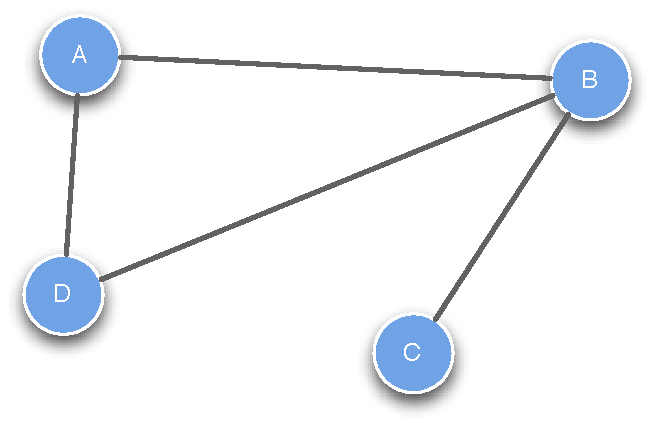
\includegraphics[width=0.45\textwidth]{assets/pdf/graph_undirected.pdf}
				}% 
	\qquad 
	\subfloat[][]{
					\label{fig:graph_undirected_weighted} %
					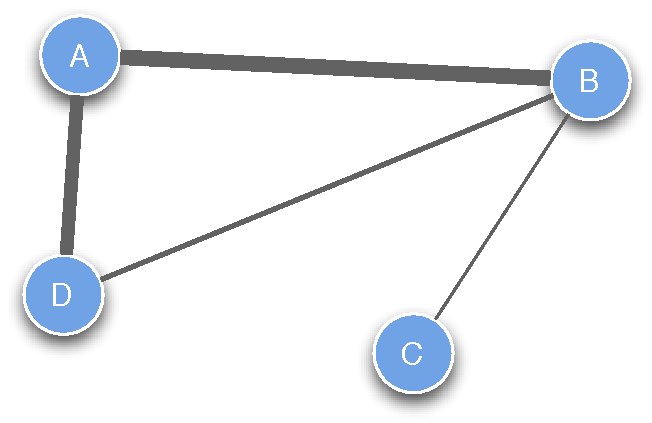
\includegraphics[width=0.45\textwidth]{assets/pdf/graph_undirected_weighted.pdf}
				} 
	\caption[Undirected model network with binary and weighted edges]{An undirected model network with binary edges \subref{fig:graph_undirected}, and the same network with weighted edges \subref{fig:graph_undirected_weighted}.} 

\end{figure}	 

Another type of networks are the so called directed networks (see figures \ref{fig:graph_directed} and \ref{fig:graph_directed_weighted}). Unlike the undirected networks, the edges have a direction (usually depicted by an arrowhead). Applied to our real world model networks, the direction could represent a one way track of a train network, or the connection between a supplier and a customer. 

\begin{figure}[htpb]% 
	\centering 
	\subfloat[][]{
					\label{fig:graph_directed} %
					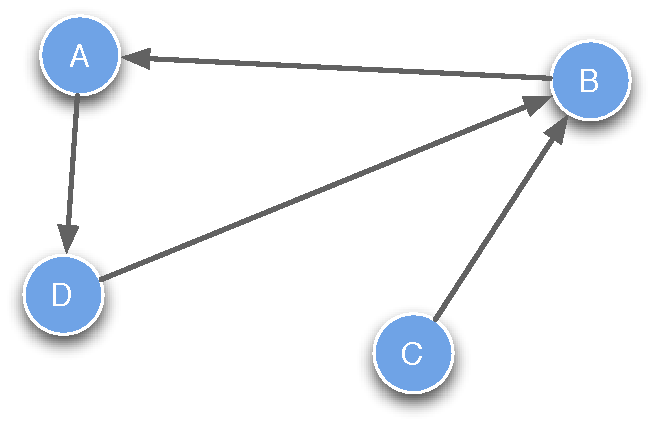
\includegraphics[width=0.45\textwidth]{assets/pdf/graph_directed.pdf}
				}% 
	\qquad 
	\subfloat[][]{
					\label{fig:graph_directed_weighted} %
					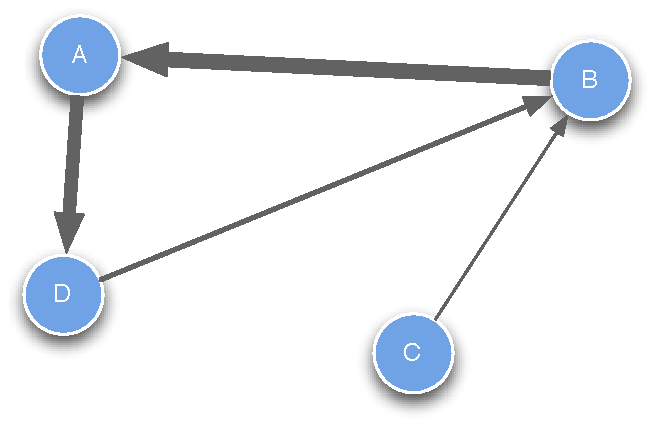
\includegraphics[width=0.45\textwidth]{assets/pdf/graph_directed_weighted.pdf}
				} 
	\caption[Directed model network with binary and weighted edges]{A directed model network with binary edges \subref{fig:graph_directed}, and the same network with weighted edges \subref{fig:graph_directed_weighted}.} 

\end{figure}

A special network is the so called \textit{Ego Network}. The ego network consists of a focal node, called the \textit{Ego}, and the nodes directly connected to \textit{Ego}, plus the edges between them. The ego network for node \textbf{A} is shown in figure \ref{fig:graph_ego}. See figure \ref{fig:graph_undirected} for the full network.	 

There are plenty of other varieties of networks. But the ones described above are adequate to understand the visualization implemented in the \textit{miceminer} application.

\subsubsection{Adjacency matrix}
\label{subsubsec:adjacency_matrix}

The data underlying the visualization is usually represented as a so called \textit{adjacency matrix}. Table \ref{tab:am_undirected} shows the tabular representation of the network shown in figure \ref{fig:graph_undirected} and the corresponding adjacency matrix alongside in figure \ref{fig:am_undirected}.

\begin{figure}[htbp]
	\begin{minipage}[t]{0.45\textwidth}
    \vspace{0pt}
		\centering
			\newcolumntype{H}{>{\bf}p{.5cm}}
			\begin{tabularx}{.5\textwidth}{+H|^X^X^X^X}
			\rowstyle{\bfseries}
				&	A	&	B	&	C	&	D \\\midrule
			A	&	0	&	1	&	0	&	1 \\
			B	&	1	&	0	&	1	&	1 \\
			C	&	0	&	1	&	0	&	0 \\
			D	&	1	&	1	&	0	&	0 \\	
			\end{tabularx}
			\captionof{table}{Tabular representation of the network shown in figure \ref{fig:graph_undirected}.}
			\label{tab:am_undirected}
	\end{minipage}
	\hspace{0.5cm}
	\begin{minipage}[t]{0.5\textwidth}
    \captionsetup{width=.5\textwidth}
    \vspace{0pt}
		\centering
		\[
		\begin{pmatrix}
        	0	&	1	&	0	&	1 \\
			1	&	0	&	1	&	1 \\
			0	&	1	&	0	&	0 \\
			1	&	1	&	0	&	0 \\
		\end{pmatrix} 
		\]
		\captionof{figure}{The adjacency matrix of the data shown in table \ref{tab:am_undirected}.}
		\label{fig:am_undirected}
	\end{minipage}
\end{figure}

For the model network with the weighted graph (figure \ref{fig:graph_undirected_weighted}) the tabular representation and the adjacency matrix looks like shown in table \ref{tab:am_undirected_weighted} and figure \ref{fig:am_undirected_weighted} (assuming that the maximum weight of an edge is 5).

An adjacency matrix for an undirected network is symmetrical by the diagonal, since the edges do not have any direction. 

\begin{figure}[ht]
	\begin{minipage}[t]{0.5\textwidth}
    \captionsetup{width=.45\textwidth}
    \vspace{0pt}
		\centering
			\newcolumntype{H}{>{\bf}p{.5cm}}
			\begin{tabularx}{.5\textwidth}{+H|^X^X^X^X}
			\rowstyle{\bfseries}
				&	A	&	B	&	C	&	D \\\midrule
			A	&	0	&	5	&	0	&	4 \\
			B	&	5	&	0	&	1	&	2 \\
			C	&	0	&	1	&	0	&	0 \\
			D	&	4	&	2	&	0	&	0 \\	
			\end{tabularx}
			\captionof{table}{Tabular representation of the network shown in figure \ref{fig:graph_undirected_weighted}.}
			\label{tab:am_undirected_weighted}
	\end{minipage}
	\hspace{0.5cm}
	\begin{minipage}[t]{0.5\textwidth}
    \captionsetup{width=.5\textwidth}
    \vspace{0pt}
		\centering
		\[
		\begin{pmatrix}
			0	&	5	&	0	&	4 \\
			5	&	0	&	1	&	2 \\
			0	&	1	&	0	&	0 \\
			4	&	2	&	0	&	0 \\	
		\end{pmatrix} 
		\]
		\captionof{figure}{The adjacency matrix of the data shown in table \ref{tab:am_undirected_weighted}.}
		\label{fig:am_undirected_weighted}
	\end{minipage}
\end{figure}

Consequently, for a directed network, as the one shown in figure \ref{fig:graph_directed}, the adjacency matrix does not show any symmetry (see table \ref{tab:am_directed} and figure \ref{fig:am_directed}).

\begin{figure}[!htpb]
	\begin{minipage}[t]{0.5\textwidth}
    \centering
    \captionsetup{width=.5\textwidth}
    \vspace{0pt}
			\newcolumntype{H}{>{\bf}p{.5cm}}
			\begin{tabularx}{.5\textwidth}{+H|^X^X^X^X}
			\rowstyle{\bfseries}
				&	A	&	B	&	C	&	D \\\midrule
			A	&	0	&	1	&	0	&	1 \\
			B	&	0	&	0	&	1	&	1 \\
			C	&	0	&	0	&	0	&	0 \\
			D	&	0	&	0	&	0	&	0 \\	
			\end{tabularx}
			\captionof{table}{Tabular representation of the network shown in figure \ref{fig:graph_directed}.}
			\label{tab:am_directed}
	\end{minipage}
	\hspace{0.5cm}
	\begin{minipage}[t]{0.5\textwidth}
    \captionsetup{width=.5\textwidth}
    \vspace{0pt}
		\centering
		\[
		\begin{pmatrix}
			0	&	1	&	0	&	1 \\
			0	&	0	&	1	&	1 \\
			0	&	0	&	0	&	0 \\
			0	&	0	&	0	&	0 \\	
		\end{pmatrix} 
		\]
		\captionof{figure}{The adjacency matrix of the data shown in table \ref{tab:am_directed}.}
		\label{fig:am_directed}
	\end{minipage}
\end{figure}

\begin{figure}[!htpb]
\begin{center}
  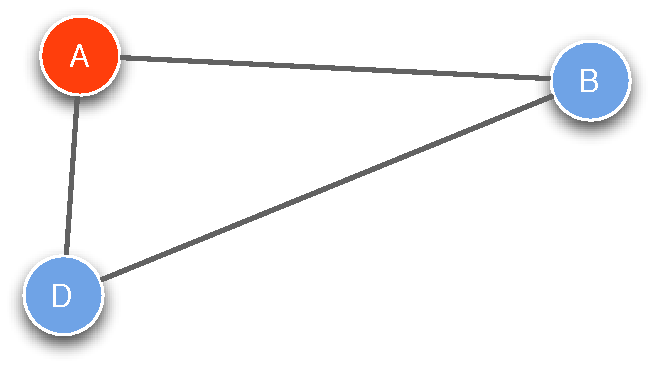
\includegraphics[width=.33\textwidth]{assets/pdf/graph_egocentric.pdf}
  \caption[Ego network]{Ego network for node \textbf{A}.}
  \label{fig:graph_ego}
\end{center}
\end{figure} 

The adjacency matrix offers the basis to apply mathematics to the network, such that networks or nodes within networks can be compared. These analytical measurements are outlined in the following section.

\subsubsection{Node based measures}
\label{subsubsec:node_based}

In order to have comparable statistical values of nodes within a network, measures are defined to quantify the degree or position of a node within a network. There are several of these so called node based measures available. Presented here are just the ones which are available in the \textit{miceminer} implementation.

The following methods to calculate the node based measures apply to networks with unweighted edges. Approaches are available, however, to calculate some of the measures for networks with weighted edges. Though, the mathematics behind these methods is quite complex and most of the software available to analyse networks do not offer these methods.

For the following explainations, the model network from the previous sections is sligthly extended, to look as shown in figure \ref{fig:extended_network}.

\begin{figure}[!htpb]
\begin{center}
  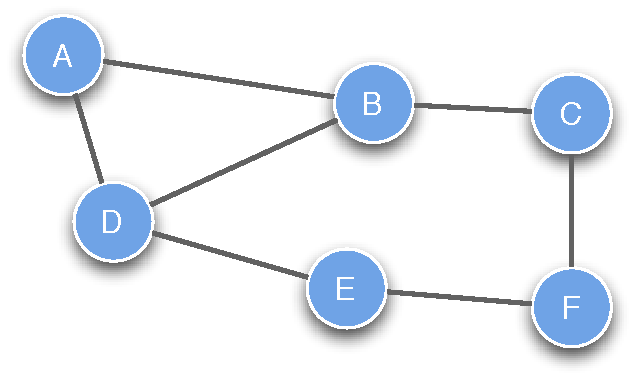
\includegraphics[width=.33\textwidth]{assets/pdf/graph_undirected_node_based.pdf}
  \caption{Extended model network}
  \label{fig:extended_network}
\end{center}
\end{figure}    

\paragraph{Average path length}

The average path length is determined by calculating the average of the shortest distances from a node to all of the other nodes. Denoting the average path length for a node $i$ as $L_i$ the equation looks as follows:

\begin{equation}
L_i = \frac{1}{(n-1)}\sum^n_{j=1} d_{ij}
\label{eq:average_path_lenght}
\end{equation}

Applied to node $E$ in the model network we get

\begin{equation}
L_E = \frac{1}{(6-1)}(2 + 2 + 2 + 1 + 0 + 1) = \frac{8}{5} = 1.6
\label{eq:average_path_lenght_e}
\end{equation}

since the distances from node $E$ to the other nodes are:

\begin{multline} 
\\d_{EA} = 2 \\
d_{EB} = 2 \\
d_{EC} = 2 \\
d_{ED} = 1 \\
d_{EE} = 0 \\
d_{EF} = 1 \\
\label{eq:distances_e}
\end{multline}

The mean path length of a network ($L$) is simply the average of all the distances within the network.

\begin{equation}
L = \frac{1}{ \frac{1}{2}n(n-1)}\sum_{i<j} d_{ij} = \frac{1}{n}\sum^n_{i=1}L_i
\label{eq:mean_path_lenght}
\end{equation} 

In a social network, this value is an indicator of how fast information can spread. The lower the value of $L$, the faster the information is received by all the individuals in the network. 

\paragraph{Clustering coefficient}

The clustering coefficient is a measure of how connected the neighborhood of a node is, and contributes to the understanding of how information in a network flows as well.

Unlike the mean path length, only the nodes which are directly connected to a node (= neighborhood) are taken into account for the calculation. To start, the existing and possible edges in the neighborhood for a certain node are determined. Shown in figure \ref{fig:clust_coeff} is the neighborhood of node \textbf{B}. Possible edges are indicated by a dotted line.

\begin{figure}[htpb]
\begin{center}
  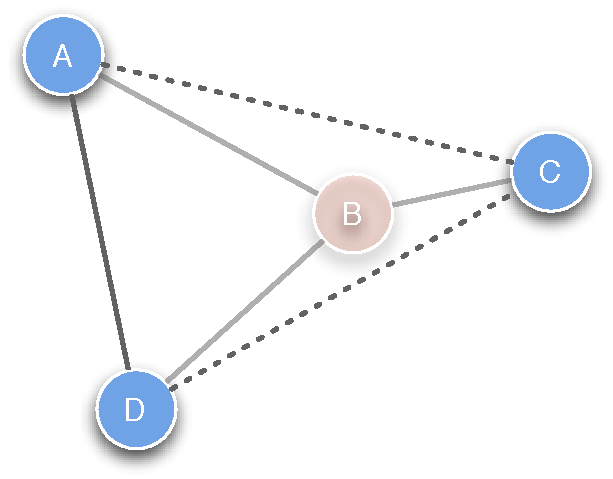
\includegraphics[width=.33\textwidth]{assets/pdf/clustering_coefficient.pdf}
  \caption[Neighborhood of node \textit{B}]{Neighborhood of node \textit{B}. Existing edges are indicated by a solid line, possible ones by a dotted line.}
  \label{fig:clust_coeff}
\end{center}
\end{figure}

In theory, the maximum number of edges in the neighborhood of a node $i$ is $\frac{1}{2}k_i(k_1 -1)$, where $k$ is the number of nodes directly connected to $i$. This makes $\frac{1}{2}3(3 -1) = 3$ for node \textbf{B}. The clustering coefficient is just the fraction of the edges between the neighborhood nodes that really exist, which is $\frac{1}{3}$. The average of the clustering coefficient of all nodes is called network clustering coefficient $C$.

\begin{equation}
C = \frac{1}{n}\sum^n_{i=1}C_i
\end{equation}  

Newman\cite{newman:2003} demonstrated, by using a model of an epidemic spreading with a fixed number of edges but adjustable clustering coefficient, that a transmissible disease could afflict a population more quickly the higher the clustering coefficient.
     
\paragraph{Degree}

The degree ($k_i$) of a node $i$ is the number of edges connected to it. This has already been used to calculate the clustering coefficient. The mean degree ($k$) is then the average of the degree of all nodes in the network.

\begin{equation}
k = \frac{1}{n}\sum_i k_i
\end{equation}

This simple to calculate measure should not be underestimated. For example, if an individual with a high degree spreads an information to the network, it will propagate much faster than if the information originates from an individual with a low degree. It is even possible that the information will never propagate to all individuals if the degree of the originator is to low.

\paragraph{Node Betweenness}

The node betweenness, written as $B_i$, is calulated by searching for all the shortest paths between two nodes, $j$ and $k$ written as $g_{jk}$, that go through node $i$, written as $g_{jik}$.

\begin{equation}
B_i =	\sum_{
			\substack{i \neq k \neq j \\ i \neq j}
		}
		\frac{g_{jik}}{g_{jk}}
\end{equation}

For node \textbf{B} in the model network shown in figure \ref{fig:node_based_measures}, $B_i = 2.5$.

Usually the betweeness values correlate with the degree. But sometimes, a node can play an important role as he connects two groups of nodes within the network as shown in figure \ref{fig:broker}. The node colored red is called a \textit{Broker}, since all the shortest paths between the nodes from the group on the left to the one on the right go through this node. In this example network, several nodes within the groups have a higher degree than the \textit{Broker}, but play a minor role when information needs to be spread over the whole network. 

\begin{figure}[htpb]
\begin{center}
  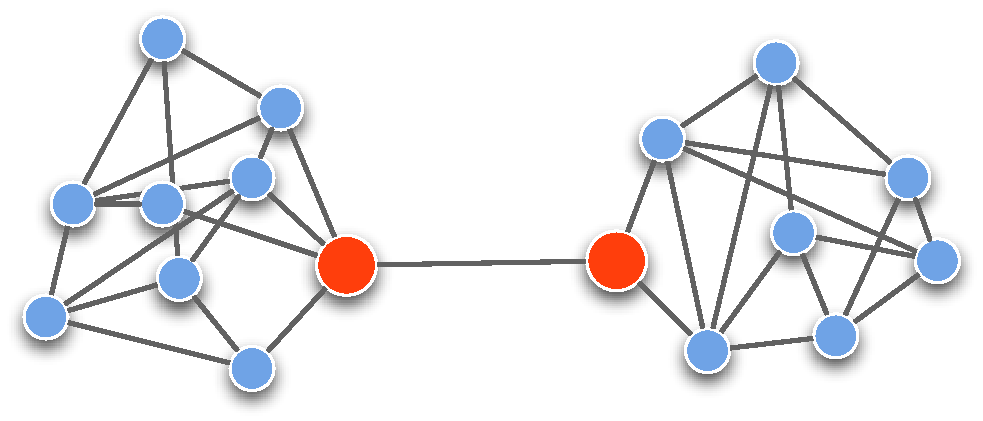
\includegraphics[width=.75\textwidth]{assets/pdf/broker.pdf}
  \caption[Model network consisting of two groups]{Model network consisting of two groups connected by single node, called a ``Broker''.}
  \label{fig:broker}
\end{center}
\end{figure}

\paragraph{Model networks}

Node based measures calculated for a network needs to be compared to some kind of a null model network, which is very well studied and understood. After all, this reveals the significant differences of a network in question to a network which is just created by chance.

Such models networks are for example the \textbf{Regular Network} (figure \ref{fig:regular_graph}), \textbf{Random Network} (figure \ref{fig:random_graph}), \textbf{Small World Network} and the \textbf{Scale-Free Networks}.

Detailed information about the properties of these model networks is beyond the scope of this document \footnote{Pages 74 - 81 in the book \textit{Exploring Animal Social Networks}\cite{croft:07} offers a good introduction to this topic.}.

\begin{figure}[htpb]% 
	\centering 
	\subfloat[][]{
					\label{fig:regular_graph} %
					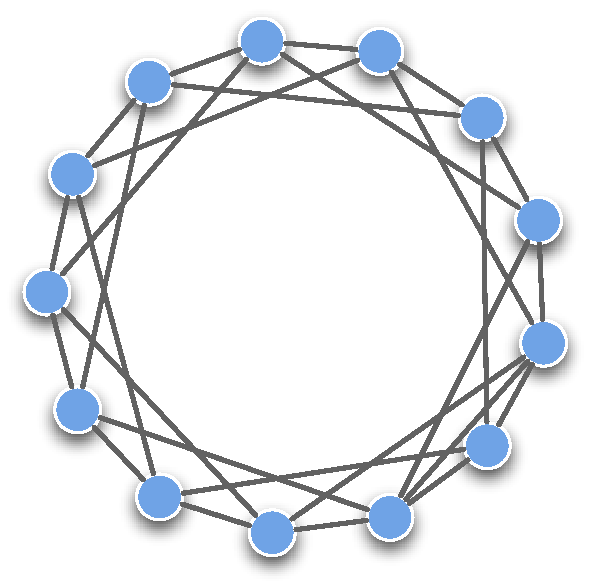
\includegraphics[width=.33\textwidth]{assets/pdf/regular_network.pdf}
				}% 
	\qquad 
	\subfloat[][]{
					\label{fig:random_graph}%
					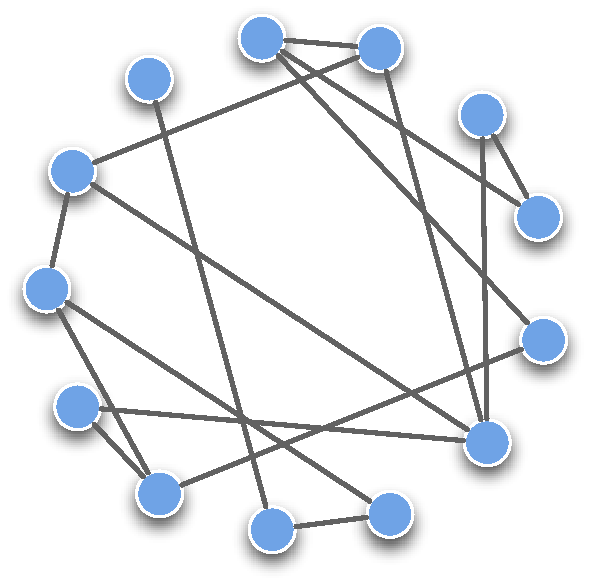
\includegraphics[width=.33\textwidth]{assets/pdf/random_network.pdf}
				} 
	\caption[A regular and a random model network]{A regular \subref{fig:regular_graph}, and a random \subref{fig:random_graph} model network with the same number of nodes.} 
	 
\end{figure} 

\subsection{Concept}
\label{subsec:graph_concept}

Social relations in the sense of this project are defined as the time two mice spend together in an artificial nestbox. This is an obvious approach. Mice only share an area at the same time voluntarily, if they have some kind of affirmative social relation.

Since the data includes information about the strength of the relationship, which is the actual time two mice spent together, the network has weighted edges. In some way, the data even includes directional information. As mentioned in the section about the meeting results, there are four different situations (meeting types) imaginable, how two mice can meet (see list \ref{list:meeting_types} and the corresponding figure \ref{fig:meeting_types}). Anyway, this information is not clearly unidirectional. Since the edges are made up of several different meetings, whereof never all of them are of the same meeting type, we do not have an exlicit directed graph.

Consequently, an undirected network with weighted edges is shown. The weight depends on the sum of time two mice spend together over a period of time. In addition, the node based measures for the shown mice and information about the composition (different meetings) of the edges must be available.

The aim was not to build a comprehensive tool for social network analysis, as there are already plenty of them available. Instead, the component is intended to provide methods to carry out data mining of the network or meeting data. Similar to the component to browse the data, the user should be provided with a tidy interface presenting the main information and options: the visualization of the network and the corresponding node based values, as well as export options for further analysis in the preferred software.

\subsection{Configuration}
\label{subsec:graph_config}

There is only one configuration value in the XML configuration file worth mentioning here. With the \lstinline|limit| value (see clipping \ref{lst:graph_data_limit} on page \pageref{lst:graph_data_limit}) one can set the minimal time, two mice must have spent together in whatever box to be included in the data which is shown by the application. 

\subsection{Implementation}
\label{subsec:graph_explore}

Pictured in figure \ref{fig:graph_data_interface_overview} is an overview of the interface for the \textbf{Graph Data} component. 

\begin{figure}[!htpb]
\begin{center}
  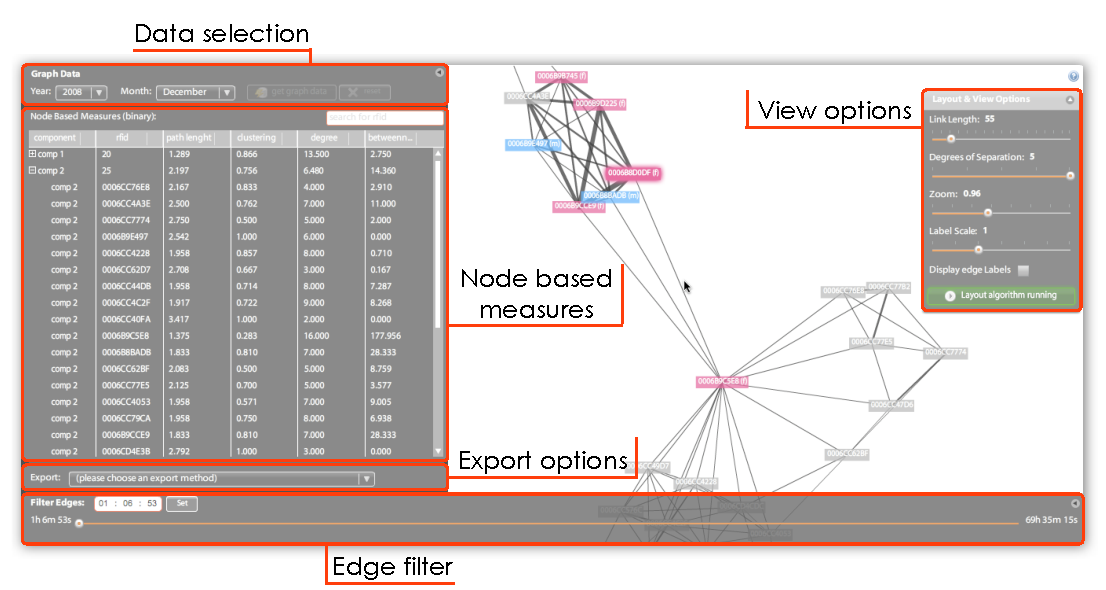
\includegraphics[width=\textwidth]{assets/pdf/graph_data_interface_overview.pdf}
  \caption[Graph Data interface overview]{Interface overview of the \textbf{Graph Data} component.}
  \label{fig:graph_data_interface_overview}
\end{center}
\end{figure}

The displayed network consist of the nodes, which are the mice, and weighted edges which denote the sum of the duration of all meeting results (see \ref{subsec:meetingres} on page \pageref{subsec:meetingres} for details), during the selected period. Female mice are colored pink, male mice light blue, and the ones without a known gender grey. 

The network can be dragged over the whole area of the component. Additionaly, the panels containing the controls and node based measures can be mimimized for an unhindered visual exploration.

Following a few details about the labeled interface parts in figure \ref{fig:graph_data_interface_overview}.

\subsubsection*{Data selection}
The period of the loaded network data is always one month\footnote{Based on the amount of data this seems to be an appropriate period.}. Month selection is done by choosing the year and a month from the respective drop down menus.  

\subsubsection*{Node based measures}

Figure \ref{fig:node_based_measures} shows a section of the table containing the mice (nodes) and their corresponding node based measures, which are:

\begin{mylist}
\item Average path length
\item Clustering coefficient
\item Degree
\item Betweenness
\end{mylist}

As it turned out, the network, consists of several unconnected network components. Due to technical limitations and performance issues, not all the components can be shown at the same time. Therefore, a mechanism to choose which network component to show had to be introduced.

The nodes in the table are grouped by the network component they belong to (see labeled pointer in figure \ref{fig:node_based_measures}). When the user clicks on the entry for a node, which is not in the network component currently visualized, the application switches to the appropriate visualization.

However, if the clicked node belongs to the currently shown component, the node will be highlighted (node gets a glow effect) and moved to the center of the visualization. This highlight mechanism works vice versa as well. If the user double-clicks a node in the visualization, the corresponding table row will be selected.

\begin{figure}[!htpb]
\begin{center}
  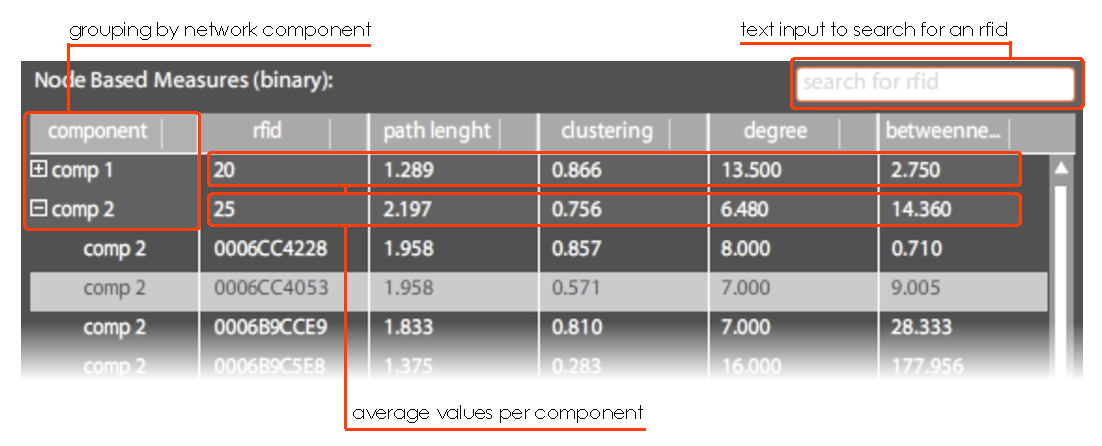
\includegraphics[width=\textwidth]{assets/pdf/node_based_measures.pdf}
  \caption[Node based measures]{Intercative table containing the node based measures.}
  \label{fig:node_based_measures}
\end{center}
\end{figure}

The second label in figure \ref{fig:node_based_measures} points to a text input with which a certain rfid (node) can be searched. This comes in escpecially handy when one tries to follow a specific mouse over different months.    

\subsubsection*{Layout \& view options}

This panel offers settings to vary the different aspects of the network visualization. Using the respective slider, the link length, the zoom level, the node size as well as the degree of separation shown can be altered. The degree of separation limits the visible nodes to a certain distance from the currently highlighted node. In addition, a checkbox is available to show or hide the edge labels.

Normally the network layout is done by a so called layouter. In this case, a force directed layouter is used, which treats the edges as they were springs. These spring forces determine the final position of a node. Consequently, nodes with a high degree are placed more in the center and the others in the periphery. At times, this can make it difficult to examine and select a node which lies in a central location, due to the entanglement of nodes and edges in this area. Therefore, the automatic layout can be switched off and the nodes can be freely dragged to a desired position.

\subsubsection*{Export options}

Since the \textit{miceminer} does not offer a full set of tools for social network analysis, an export to a file format, which can be imported into \textit{NetDraw} or \textit{UCINET}\footnote{Visit \href{http://www.analytictech.com/downloadnd.htm}{http://www.analytictech.com/downloadnd.htm} for details.}, is available. \textit{NetDraw} is a versatile tool to visualize networks, whereas \textit{UCINET} offer comprehensive methods for social network analysis. Shown in figure \ref{fig:netdraw_export_component} is a screenshot of \textit{NetDraw} visualizing a network for which the data has been exported from the \textit{miceminer} application.

\begin{figure}[htpb]
\begin{center}
  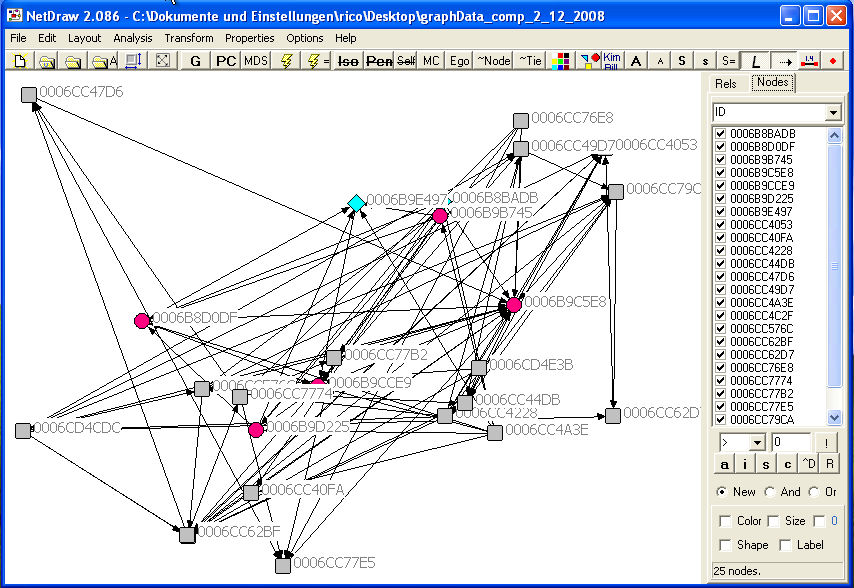
\includegraphics[width=\textwidth]{assets/img/netdraw_export_component.png}
  \caption[Scereenshot of the Netdraw application]{Screenshot of the \textit{NetDraw} application visualizing a network.}
  \label{fig:netdraw_export_component}
\end{center}
\end{figure}

The edge data, as well as the node based measures, can be exported to an \textit{Excel} worksheet. Additionally, the network visualization can be exported as an image.

\subsubsection*{Edge filter}

Edge filtering is used to hide edges which are under a certain weight. This can reveal social groups which are strongly connected within a network component, or highlight edges that are more likely to be nonrandom.

\subsubsection*{Additional options}

A few additional options, that turned out to be useful or were just implemented out of interest, have been added to the component.

\paragraph{Egocentric network view}

Switching to the egocentric network view can be useful to verify a thesis about the importance of an individual in the network. In addition, when the egocentric view has been activated (by holding the \lstinline|Shift| key while clicking on the highlighted node), the user can choose another node from within the egocentric network of the starting node, to check the egocentric network of this node.

\paragraph{Edge data}

To unveil the \lstinline|meeting results| which make up an edge, the label of the edges can be double clicked. A pop up window will open, containing the meeting data, which can be explored either in a tabular or in a chart view, similar to the interface of the \textbf{Browse Data} component.

In the tabular view, the data can be grouped by the nestboxes, the meetings took place in, or by the meeting type\footnote{See list \ref{list:meeting_types} on page \pageref{list:meeting_types} for details about the meeting types.}.

The chart view is used to bin the data by the meeting duration. The number of bins can be adjusted, and the grouping of the data can be set to the nestboxes or meeting type (see figure \ref{fig:edge_data_panel_chart}).

\begin{figure}[!htpb]
\begin{center}
  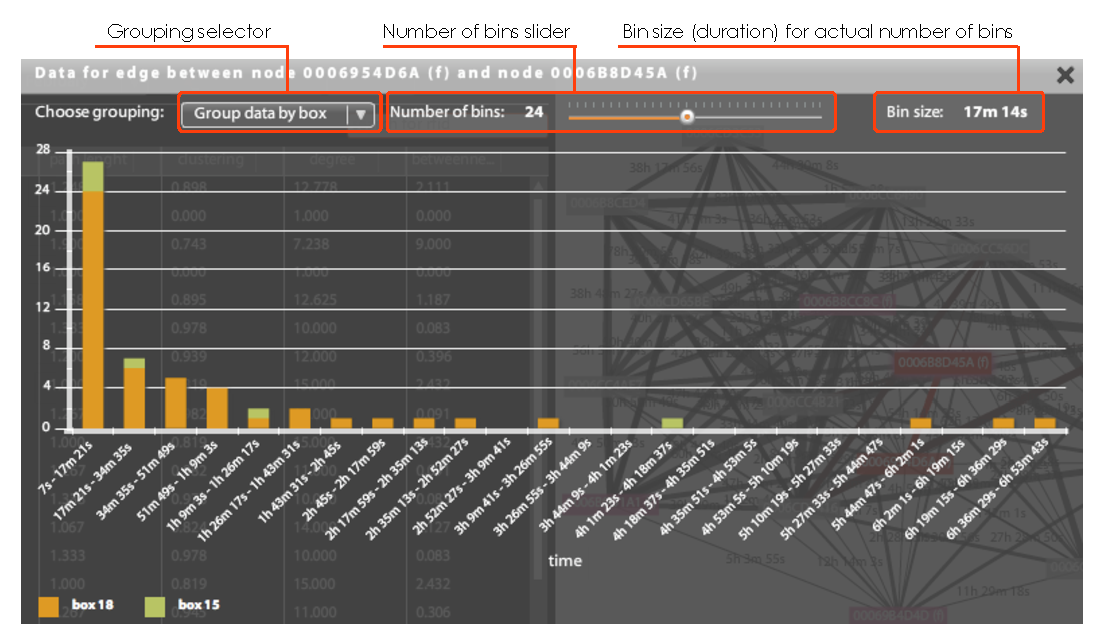
\includegraphics[width=\textwidth]{assets/pdf/edge_data_panel_chart.pdf}
  \caption[Edge data chart]{Chart of the binned \lstinline|meeting results|, grouped by the nestbox which make up an edge between the mice with rfid \lstinline|0006954D6A| and \lstinline|0006B8D45A|.}
  \label{fig:edge_data_panel_chart}
\end{center}
\end{figure}   

\subsection{Possible research}
\label{subsec:graph_research}
